\documentclass[tikz,border=10pt]{standalone}

\usepackage{tikz}
\usetikzlibrary{positioning}
\usetikzlibrary{shapes,arrows,backgrounds,fit,shapes.geometric,calc}
\usetikzlibrary{pgfplots.groupplots}
\usepackage{pgfplots}
\usepackage{pgfplotstable}
\usepackage{listings}
\usepackage{lstautogobble}
\usepackage{color}
\usepackage{amsmath}

\lstset{
    language=[ANSI]C++,
    basicstyle=\small\ttfamily,
    identifierstyle=\color{black}\small\ttfamily,
    keywordstyle=\color{red}\small\ttfamily,
    commentstyle=\color{green!30!black}\bf\small\ttfamily,
    breaklines=true
}

\tikzset{
    %Define standard arrow tip
    >=stealth',
    % Define arrow style
    pil/.style={
           ->,
       thick,}
           %shorten <=2pt,
           %shorten >=2pt,}
}

\newcommand{\itemheight}{0.75cm}

\begin{document}
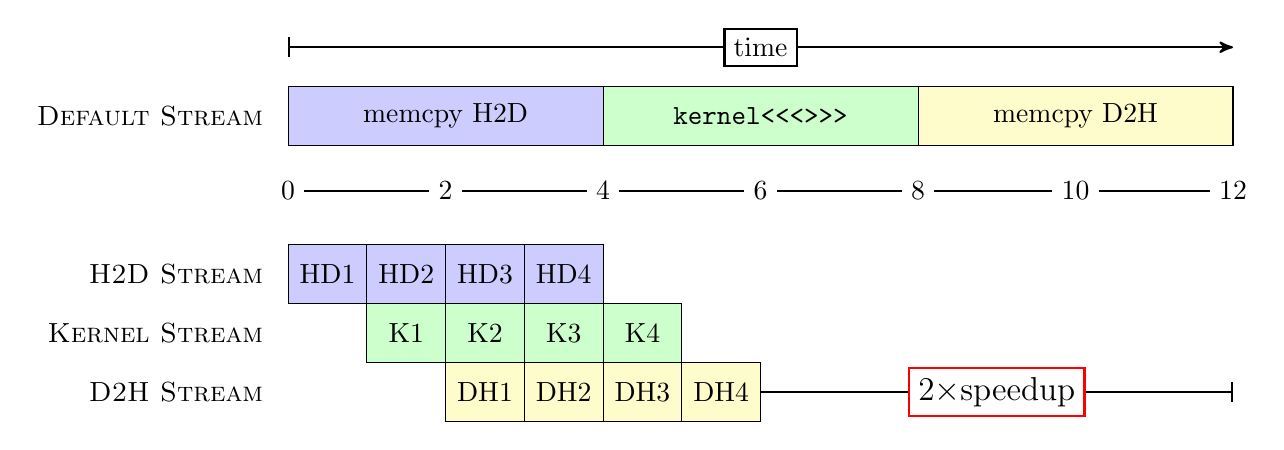
\begin{tikzpicture}[x=0cm, y=0cm, node distance=0 cm,outer sep = 0pt]
\tikzstyle{h2d}=[
                  draw=black,
                  rectangle,
                  minimum height=\itemheight,
                  fill=blue!20,
                  anchor=north west]

\tikzstyle{kernel}=[
                  draw=black,
                  rectangle,
                  minimum height=\itemheight,
                  fill=green!20,
                  anchor=north west]

\tikzstyle{d2h}=[
                  draw=black,
                  rectangle,
                  minimum height=\itemheight,
                  fill=yellow!20,
                  anchor=north west]

\coordinate (a) at (0cm, 0.5cm);
\coordinate (b) at (12cm,0.5cm);
\draw [|->,thick] (a) -- (b) node [midway,fill=white,draw] {time};

\node[h2d]   (h2dfull)    at(0,0) [minimum width=4cm]                        {memcpy H2D};
\node[kernel](kernelfull)         [right = of h2dfull, minimum width=4cm]    {\verb!kernel<<<>>>!};
\node[d2h]   (d2hfull)            [right = of kernelfull, minimum width=4cm] {memcpy D2H};

\node[rectangle] (snull) [left=0.2cm of h2dfull] {\sc Default Stream};

\node[h2d]   (h2d1) at(0,-2cm) [minimum width=1cm]                {HD1};
\node[h2d]   (h2d2)            [right = of h2d1, minimum width=1cm] {HD2};
\node[h2d]   (h2d3)            [right = of h2d2, minimum width=1cm] {HD3};
\node[h2d]   (h2d4)            [right = of h2d3, minimum width=1cm] {HD4};

\node[kernel] (kernel1) [below = of h2d2, minimum width=1cm]    {K1};
\node[kernel] (kernel2) [right = of kernel1, minimum width=1cm] {K2};
\node[kernel] (kernel3) [right = of kernel2, minimum width=1cm] {K3};
\node[kernel] (kernel4) [right = of kernel3, minimum width=1cm] {K4};

\node[d2h] (d2h1) [below = of kernel2, minimum width=1cm] {DH1};
\node[d2h] (d2h2) [right = of d2h1, minimum width=1cm]    {DH2};
\node[d2h] (d2h3) [right = of d2h2, minimum width=1cm]    {DH3};
\node[d2h] (d2h4) [right = of d2h3, minimum width=1cm]    {DH4};

\coordinate (t0)  at (0cm,-1.325cm);
\coordinate (t2)  at (2cm,-1.325cm);
\coordinate (t4)  at (4cm,-1.325cm);
\coordinate (t6)  at (6cm,-1.325cm);
\coordinate (t8)  at (8cm,-1.325cm);
\coordinate (t10) at (10cm,-1.325cm);
\coordinate (t12) at (12cm,-1.325cm);

\draw [|-|,thick] (t0) -- (t12);
\node[rectangle] at(t0) [fill=white] {0};
\node[rectangle] at(t2) [fill=white] {2};
\node[rectangle] at(t4) [fill=white] {4};
\node[rectangle] at(t6) [fill=white] {6};
\node[rectangle] at(t8) [fill=white] {8};
\node[rectangle] at(t10) [fill=white] {10};
\node[rectangle] at(t12) [fill=white] {12};

\coordinate (c) at (6cm, -3.875cm);
\coordinate (d) at (12cm,-3.875cm);
\draw [.-|,thick] (c) -- (d) node [midway,fill=white,draw=red] {\large 2$\times$speedup};

%\draw [-,thick,black!40] (6cm,-1.5cm) -- (6cm,-3.4cm);

\node[rectangle] (sh2d)    [left=0.2cm of h2d1]     {\sc H2D Stream};
\node[rectangle] (skernel) [left=1.2cm of kernel1]  {\sc Kernel Stream};
\node[rectangle] (sd2h)    [left=2.2cm of d2h1]     {\sc D2H Stream};

\end{tikzpicture}

\end{document}

